\chapter{A first look at the problem}\label{cha:first-look}

Problem, general calculations from Julens paper without casimir

When is the system entangled (distance-measures, fidelity ??)

\begin{figure}[!htbp]
  \centering
  \def\svgwidth{\textwidth}
  \input{./../figures/simple-problem.pdf_tex}
  \caption{Simple Problem from Julens paper}
\end{figure}

Ignoring (for now) all other forms of interaction between the masses except gravity

The density $\rho(t) = \ketbra{\psi(t)}$ can be represented in the basis $\left\{ \ket{\psi_A^\uparrow}, \ket{\psi_A^\downarrow} \right\}\otimes \left\{ \ket{\psi_B^\uparrow}, \ket{\psi_B^\downarrow} \right\}$ as
\begin{equation}
  \rho(t) = \frac{1}{4}
  \begin{pmatrix}
    1 &   &   & 1 \\
      & 1 &   &   \\
      &   & 1 &   \\
    1 &   &   & 1
  \end{pmatrix}
\end{equation}


\section{Entanglement measures}
Why are they needed, what can one do?

Logarithmic negativity, properties, calculation





\begin{figure}[!htbp]
  \centering
  \def\svgwidth{0.9\textwidth}
  \input{./../figures/problem-geometry.pdf_tex}
  \caption{My problem}
\end{figure}


\begin{figure}[!htbp]
  \centering
  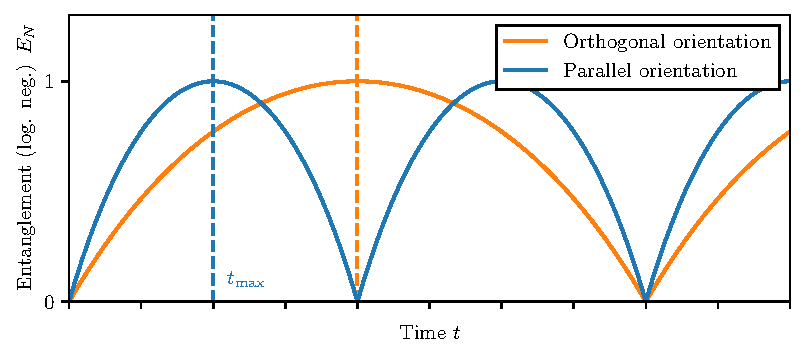
\includegraphics[width=\textwidth]{./../figures/entanglement-time-orientation.pdf}
  \caption{Entanglement dynamics quantified by the logarithmic negativity for two different orientations of the spatial superpositions relative to each other. The time of maximum entanglement $t_\mathrm{max}$ for the parallel configuration is given by $t_\mathrm{max} = 8\pi\hbar L^3 / (G M_A M_B d^2) \simeq 258\si{ms}$.}
\end{figure}